\documentclass[11pt]{article}

\usepackage[margin=1in]{geometry}
\usepackage{amsmath,amssymb,bm}
\usepackage{tikz}
\usetikzlibrary{arrows.meta,positioning}

% --- Notation helpers (match handwritten style) ---
\newcommand{\Ind}{\mathbf{I}} % indicator function (bold I)
\newcommand{\Ber}{\mathrm{Ber}}
\newcommand{\BetaDist}{\mathrm{Beta}}
\newcommand{\Prb}{\Pr}

\title{Dose Finding Trail Design}
\author{}
\date{}

\begin{document}
\maketitle

\section*{1. Mediator factorization}

Let $d\in\{d_1,\ldots,d_J\}$ denote the assigned dose/arm, and consider the triple
\[ [Y_I,\,Y_T,\,Y_E\mid d]. \]
The factorization with a mediator $Y_I$ is
\begin{align*}
\Prb(Y_I,Y_T,Y_E\mid d)
&=\Prb(Y_I\mid d)\,\Prb(Y_T,Y_E\mid Y_I,d)\\
&=\Prb(Y_I\mid d)\,\Prb(Y_T\mid Y_I,d)\,\Prb(Y_E\mid Y_I,d).
\end{align*}
\noindent\textbf{Causal diagram (as drawn):} $d\to Y_I$, $Y_I\to Y_T$, $Y_I\to Y_E$, and direct arrows $d\to Y_T$, $d\to Y_E$.

\section*{2. Immune response model (Beta--Bernoulli)}

For dose level $j$:
\[
Y_{Ii}\mid \pi_{Ij}\sim \Ber(\pi_{Ij}),\qquad
\pi_{Ij}\sim \BetaDist(\alpha_{Ij},\beta_{Ij}).
\]
Define
\[
r_{Ij}=\sum_i Y_{Ii}\,\Ind(d_i=d_j),\qquad
n_j=\sum_i \Ind(d_i=d_j).
\]
Then
\[
\pi_{Ij}\mid \text{data}\sim \BetaDist\big(r_{Ij}+\alpha_{Ij},\;n_j-r_{Ij}+\beta_{Ij}\big).
\]
\noindent\textbf{PAVA:} transform posterior draw (to enforce monotonicity across dose).

\section*{3. Toxicity conditional on the mediator level $I\in\{0,1\}$}

For $I\in\{0,1\}$ and dose $j$:
\[
Y_{Ti}\mid (Y_{Ii}=I),\ \pi_{Tj}^{(I)}\sim \Ber\big(\pi_{Tj}^{(I)}\big),
\qquad
\pi_{Tj}^{(I)}\sim \BetaDist\big(\alpha_{Tj}^{(I)},\beta_{Tj}^{(I)}\big).
\]
Define the stratum-specific counts
\[
r_{Tj}^{(I)}=\sum_i \Ind(Y_{Ii}=I)\,\Ind(d_i=d_j)\,Y_{Ti},
\qquad
n_j^{(I)}=\sum_i \Ind(Y_{Ii}=I)\,\Ind(d_i=d_j).
\]
Then the conjugate posterior is
\[
\pi_{Tj}^{(I)}\mid \text{data}\sim
\BetaDist\Big(r_{Tj}^{(I)}+\alpha_{Tj}^{(I)},\;n_j^{(I)}-r_{Tj}^{(I)}+\beta_{Tj}^{(I)}\Big).
\]

\subsection*{Bivariate isotonic regression constraints (toxicity)}
After isotonic adjustment (denote adjusted quantities by $\tilde{\pi}$), the constraints are
\[
\tilde{\pi}_{T1}^{(0)}\le \cdots \le \tilde{\pi}_{TJ}^{(0)},\qquad
\tilde{\pi}_{T1}^{(1)}\le \cdots \le \tilde{\pi}_{TJ}^{(1)},\qquad
\tilde{\pi}_{Tj}^{(0)}\le \tilde{\pi}_{Tj}^{(1)}\ \ (j=1,\ldots,J).
\]
\begin{figure}[h]
\centering
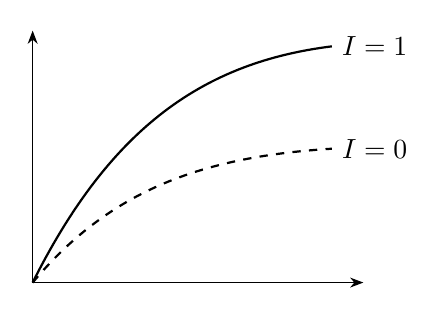
\begin{tikzpicture}[>=Stealth]
  \draw[->] (0,0) -- (4.2,0);
  \draw[->] (0,0) -- (0,3.2);

  % solid curve: I=1
  \draw[thick] (0,0) .. controls (1.0,2.0) and (2.2,2.8) .. (3.8,3.0)
    node[right] {$I=1$};

  % dashed curve: I=0
  \draw[thick,dashed] (0,0) .. controls (1.0,1.2) and (2.2,1.6) .. (3.8,1.7)
    node[right] {$I=0$};
\end{tikzpicture}
\caption{Sketch of response curves for $I=1$ (solid) vs $I=0$ (dashed).}
\end{figure}


\section*{4. Efficacy conditional on the mediator level $I\in\{0,1\}$}

\noindent (As written in the notes, $d_i=j$ indicates the subject is assigned to arm $j$.)

\[
r_{Ej}^{(I)}
= \sum_i \Ind(Y_{Ii}=I)\,\Ind(d_i=j)\,Y_{Ei},
\qquad
n_j^{(I)}=\sum_i \Ind(Y_{Ii}=I)\,\Ind(d_i=j).
\]
\[
Y_{Ei}^{(I)} \mid Y_{Ii}=I,\ \bar{\pi}_{Ej}^{(I)}
\sim \Ber\!\big(\bar{\pi}_{Ej}^{(I)}\big).
\]
\[
\bar{\pi}_{Ej}^{(I)} \mid \text{data} \sim
\BetaDist\!\Big(
  r_{Ej}^{(I)}+\alpha_{Ej}^{(I)},
  \ n_j^{(I)}-r_{Ej}^{(I)}+\beta_{Ej}^{(I)}
\Big).
\]

\subsection*{Bivariate isotonic regression constraints (efficacy)}
After isotonic adjustment (denote adjusted quantities by $\tilde{\pi}$), the constraints are
\[
\tilde{\pi}_{E1}^{(0)}\le \cdots \le \tilde{\pi}_{EJ}^{(0)},\qquad
\tilde{\pi}_{E1}^{(1)}\le \cdots \le \tilde{\pi}_{EJ}^{(1)},\qquad
\tilde{\pi}_{Ej}^{(0)}\le \tilde{\pi}_{Ej}^{(1)}\ \ (j=1,\ldots,J).
\]

\section*{5. Marginalization (mixture over $Y_I$)}

For toxicity at dose $d_j$:
\begin{align*}
\Prb(Y_T=1\mid d_j)
&=\Prb(Y_I=1\mid d_j)\,\Prb(Y_T=1\mid Y_I=1,d_j)\\
&\quad +\Prb(Y_I=0\mid d_j)\,\Prb(Y_T=1\mid Y_I=0,d_j).
\end{align*}

\noindent For a posterior draw $s$ (plug-in form as in the notes):
\[
\tilde{\pi}_{Tj}[s]
=\tilde{\pi}_{Ij}[s]\cdot \tilde{\pi}_{Tj}^{(1)}(s)
+\big(1-\tilde{\pi}_{Ij}[s]\big)\cdot \tilde{\pi}_{Tj}^{(0)}(s).
\]
\noindent Similar for efficacy:
\[
\tilde{\pi}_{Ej}[s]
=\tilde{\pi}_{Ij}[s]\cdot \tilde{\pi}_{Ej}^{(1)}(s)
+\big(1-\tilde{\pi}_{Ij}[s]\big)\cdot \tilde{\pi}_{Ej}^{(0)}(s).
\]

\end{document}
